\newpage
\subsection{Connecting your classes}
\visHeader
\hypertarget{static:references vis}{}

\begin{itemize}

\item[$\blacktriangleright$] A fundamental gesture in EA is \emph{Quick Link}. Quick Link is used to create links between elements in a context-sensitive
manner. To use Quick Link, choose an element and note the little black arrow in its top-right corner (Fig.~\ref{fig:quicklink}).

\begin{figure}[htbp]
	\centering
  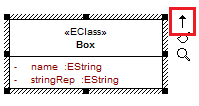
\includegraphics[width=0.4\textwidth]{ea_quickLink}
	\caption{Quick Link is a central gesture in EA}
	\label{fig:quicklink}
\end{figure}
\FloatBarrier

Click on this black arrow and `pull' to another element you wish to link to. To start, quick link from \texttt{Box} to \texttt{Partition}. In the context-menu
that pops up, choose \texttt{Create Bidirectional EReference} (Fig.~\ref{fig:ereference}).

\begin{figure}[htbp]
	\centering
  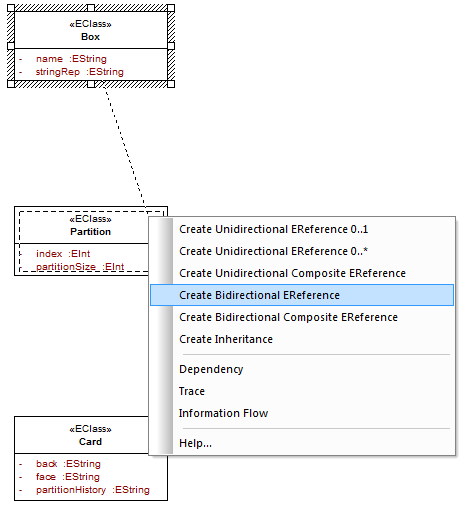
\includegraphics[width=0.5\textwidth]{ea_eReferenceBidirectional}
	\caption{Create a reference via Quick Link}
	\label{fig:ereference}
\end{figure}
\FloatBarrier

\item[$\blacktriangleright$] Double click the reference to invoke a dialogue. Here you can change the reference direction\footnote{this is particuluary useful
if you accidentally click one of the other options while creating the quick link and wish to change it, or if you went backwards from partition to box.} and
enter a name. The name will only be used for documentation purposes as it is not relevant for code generation.

\item[$\blacktriangleright$] In the same dialogue, choose \texttt{Target Role} and enter the values in Fig.~\ref{fig:reference_ends} to set the properties for
the ``target'' end of the reference (the \texttt{Box} role). As you can see, the default target is set to the class you linked \emph{from}, and the default
source is the class you linked \emph{to}. If you decided to ignore the instructions, and went from \texttt{Partition} to \texttt{Box}, the only difference
between the references are the titles - the following information will still be the same! In this window, it's important not to forget to check and modify the
\texttt{Role}, \texttt{Navigability}, \texttt{Multiplicity}, and \texttt{Aggregation} settings for the target.  Repeat the process for the \texttt{Source Role}.


\begin{figure}[htbp]
	\centering
	  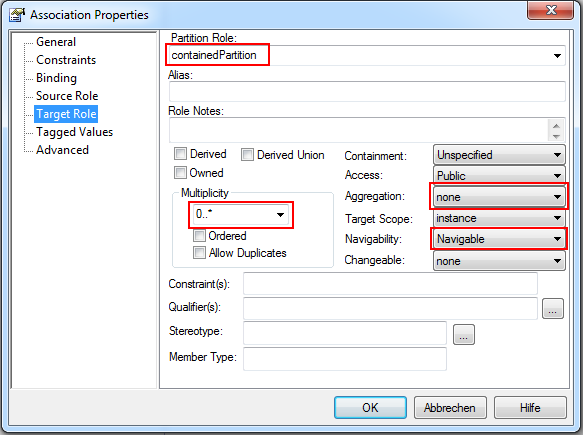
\includegraphics[width=0.73\textwidth]{ea_assocPropsTarget}\\
  \vspace{1cm}
    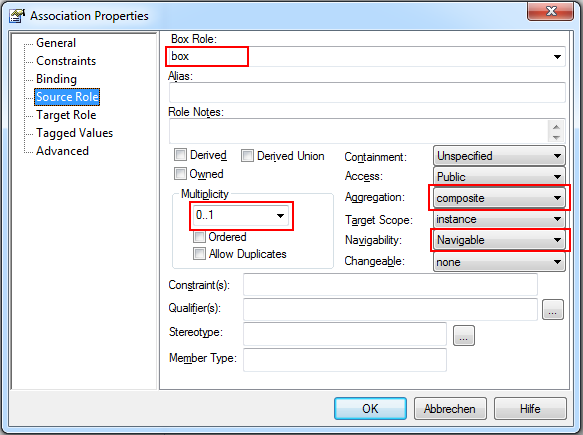
\includegraphics[width=0.73\textwidth]{ea_assocPropsSource}
	\caption{Enter properties for target and source of reference}
	\label{fig:reference_ends}
\end{figure}
\FloatBarrier


We reviewed the source and target purposes, but what are the other three options we had to modify? Firstly, navigable ends are mapped to class attributes with
getters and setters in Java and therefore \emph{must} have a specified name and  multiplicity for successful code generation. Corresponding values for
non-navigable ends can  be regarded as additional documentation and do not have to be specified.

Next, the multiplicity of a reference controls if the relation is mapped to a Java Collection (\texttt{*},  \texttt{1..*}, \texttt{0..*}), or to a single valued
class attribute (\texttt{1}, \texttt{0..1}).

Finally, in Ecore, the aggregation values of a reference can either be \texttt{none} or \texttt{com\-po\-site}. Composite means that the current role is that of
a \emph{container} for the opposite role.
In our case for example, \texttt{box} is a container for \texttt{partitions}.\\
This has a series of consequences: (1) every element must have a container, (2) an element cannot be in more than one container at the same time, and (3) a
container's contents are deleted together with the container. Non-composite (\texttt{none}) means that the current role is not that of a container and the rules
for containment do not hold (reference is a simple ``pointer'').


\item[$\blacktriangleright$] If you've done everything right, your workspace should now resemble Fig.~\ref{fig:ereference_completed} with a relation between
\texttt{Box} and \texttt{Partition}.

\begin{figure}[htbp]
	\centering
  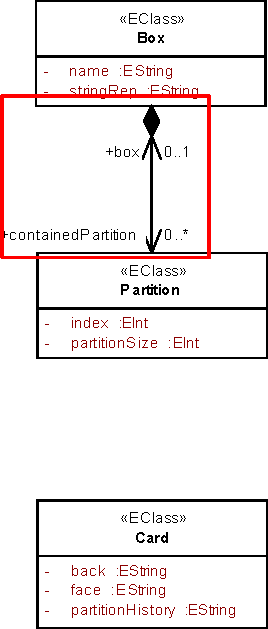
\includegraphics[width=0.3\textwidth]{ea_relationBoxPartition.pdf}
	\caption{\texttt{Box} contains \texttt{Partition}s}
	\label{fig:ereference_completed}
\end{figure}
\FloatBarrier


\item[$\blacktriangleright$] Create another bidirectional reference\footnote{To be precise, \emph{all} references in Ecore are actually unidirectional.
A ``bidirectional'' reference in our metamodel is in reality mapped to two \texttt{EReferences} that are opposites of each other.
We however believe it is simpler to handle these pairs as single references and prefer this concise concrete syntax.} between \texttt{Partition} and
\texttt{Card}, then two unidirectional self-references for \texttt{Partition} according to Fig.~\ref{fig:ereferences_all}\footnote{If you have difficulties
deciphering the role names and other details in this screenshot, please forward to figure~\ref{fig:metamodel_complete} for a better diagram of the metamodel.}.

\begin{figure}[htbp]
	\centering
  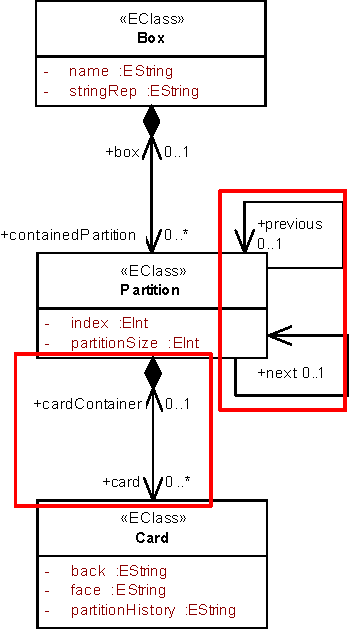
\includegraphics[width=0.5\textwidth]{ea_relationsAll.pdf}
	\caption{All relations in our metamodel}
	\label{fig:ereferences_all}
\end{figure}

\FloatBarrier

\item[$\blacktriangleright$] All of your program attributes and references have now been set up. To see how this would appear in eMoflon's textual syntax, check
out figures~\ref{fig:allReferences} and \ref{fig:partitionReferences} in \hyperlink{sec:static tex}{section 2.2}!

\fancyfoot[R]{$\triangleright$ \hyperlink{static:methods vis}{Next}}

\end{itemize}
